\documentclass[tikz,border=2pt]{standalone}
\renewcommand{\familydefault}{\sfdefault}
\usetikzlibrary{arrows.meta,calc,positioning}
\tikzset{every picture/.style={line width=1pt, >=Stealth},
         hl/.style={fill=black, fill opacity=0.12, text opacity=1}}
\begin{document}
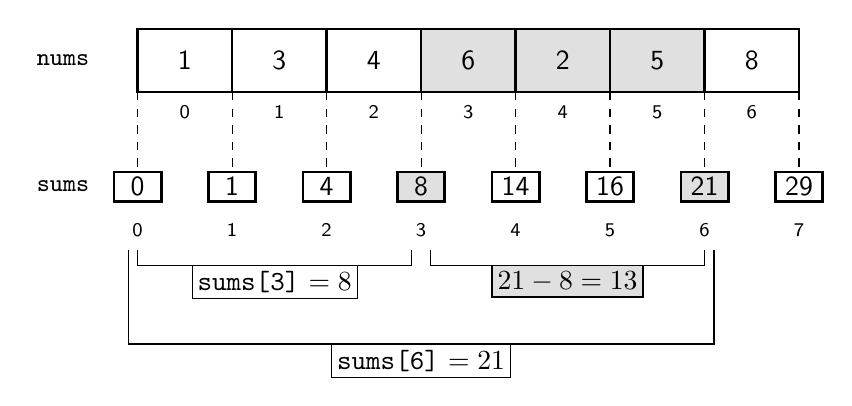
\begin{tikzpicture}[x=1.2cm, y=1cm, cell/.style={draw, minimum width=1.2cm, minimum height=0.8cm},
    sum/.style={draw, minimum width=0.6cm, inner sep=2pt}, idx/.style={font=\scriptsize}]
  % nums[i] spans [i, i + 1]; sums[k] sits on boundary k and is the sum of nums[0..k).
  \node[left, font=\small] at (-0.4, 0) {\texttt{nums}};
  \foreach \v/\s [count=\i from 0] in {1/, 3/, 4/, 6/hl, 2/hl, 5/hl, 8/} {
    \node[cell, \s] at (\i + 0.5, 0) {\v};
    \node[idx] at (\i + 0.5, -0.65) {\i};
  }
  \node[left, font=\small] at (-0.4, -1.6) {\texttt{sums}};
  \foreach \v/\s [count=\k from 0] in {0/, 1/, 4/, 8/hl, 14/, 16/, 21/hl, 29/} {
    \draw[thin, dashed] (\k, -0.4) -- (\k, -1.35);
    \node[sum, \s] at (\k, -1.6) {\v};
    \node[idx] at (\k, -2.15) {\k};
  }
  % sums[6] - sums[3] = nums[3] + nums[4] + nums[5]
  \draw[thin] (0, -2.4) -- (0, -2.6) -- node[below, sum] {\texttt{sums[3]} $= 8$} (2.9, -2.6) -- (2.9, -2.4);
  \draw[thin] (3.1, -2.4) -- (3.1, -2.6) -- node[below, sum, hl] {$21 - 8 = 13$} (6, -2.6) -- (6, -2.4);
  \draw[thin] (-0.1, -2.4) -- (-0.1, -3.6) -- node[below, sum] {\texttt{sums[6]} $= 21$} (6.1, -3.6) -- (6.1, -2.4);
\end{tikzpicture}
\end{document}
